\section{Auswertung}
\label{sec:Auswertung}
\subsection{Vorbereitung}
Für die Vorbereitung soll das Dispersionsgebiet und das Auflösungsvermögen für die beiden 
verwendeten Wellenlängen bestimmt werden. Diese Größen können mit den Gleichungen \eqref{eq:del_Lam} und \eqref{eq:del_A} berechnet werden.
Die Ergebnisse sind in Tabelle \ref{tab:Vorbereitung} aufgelistet.
\FloatBarrier
\begin{table}
    \centering
    \caption{Dispersionsgebiet und Auflösungsvermögen für die beiden Wellenlängen.}
    \label{tab:Vorbereitung}
    \begin{tabular}{c c c}
        \toprule
        Wellenlänge $\lambda$ / $\SI{}{\nano\meter}$&Auflösungsvermögen $A$& Dispersionsgebiet $\Delta \lambda_{\text{D}}$ / $\SI{}{\pico\meter}$\\
        \midrule
        rot $\num{643.8}$&$\num{2.09e5}$&$\num{48.9}$\\
        blau $\num{480.0}$&$\num{2.85e5}$&$\num{27.0}$\\
        \bottomrule
    \end{tabular}
\end{table}
\FloatBarrier
Die Quantenzahlen und die mit Gleichung \eqref{len5} berechneten Landé-Faktoren sind in Tabelle \ref{tab:Quantenzahlen} 
aufgelistet.
\FloatBarrier
\begin{table}
    \centering
    \caption{Quantenzahlen und Landé-Faktoren der einzelnen Zustände.}
    \label{tab:Quantenzahlen}
    \begin{tabular}{c c c c c}
        \toprule
        Zustand&S&L&J&$g_{\text{j}}$\\
        \midrule
        $^1\text{P}_1$&0&1&1&1\\
        $^1\text{D}_1$&0&2&2&1\\
        $^3\text{S}_1$&1&0&1&2\\
        $^3\text{P}_1$&1&L&1&$\num{1.5}$\\
        \bottomrule
    \end{tabular}
\end{table}
\FloatBarrier
Die Landé-Faktoren $g_{\text{ij}}$ der Übergänge werden mit der Gleichung \eqref{eq:Landeübergang} bestimmt.
\begin{equation}
    \label{eq:Landeübergang}
    g_{\text{ij}} = m_{\text{i}}g_{\text{i}} - m_{\text{j}}g_{\text{j}}
\end{equation}
Der Übergang des roten Lichtes ist $^1\text{P}_1 \rightarrow ^1\text{D}_1$ und für das 
blau Licht ist der Übergang $^3\text{S}_1 \rightarrow ^3\text{P}_1$.
Die Landé-Faktoren $g_{\text{ij}}$ der Übergänge des roten Lichtes sind in Tabelle \ref{tab:rotÜber} und die
für das blaue Licht in Tabelle \ref{tab:blauÜber} aufgelistet.
\FloatBarrier
\begin{table}
    \centering
    \caption{Landé-Faktoren der Zustände und Übergänge des roten Lichtes.}
    \label{tab:rotÜber}
    \begin{tabular}{c| c c| c c| c c}
        \toprule
        Übergang&\multicolumn{2}{c|}{Zustand i}&\multicolumn{2}{c|}{Zustand i}&\\
                &\multicolumn{2}{c|}{$^1\text{P}_1$}&\multicolumn{2}{c|}{$^1\text{D}_1$}&\\
        \midrule
        &$m_\text{i}$&$g_\text{i}$&$m_\text{j}$&$g_\text{j}$&$\Delta m $&$g_{\text{ij}}$\\
        \midrule
        \multirow{3}{*}{$\pi$}&1&\multirow{3}{*}{1}&1&\multirow{3}{*}{1}&\multirow{3}{*}{0}&\multirow{3}{*}{0}\\
        &0&&0&&&\\
        &-1&&-1&&&\\
        \hline
        \multirow{3}{*}{$\sigma^-$}&2&\multirow{3}{*}{1}&1&\multirow{3}{*}{1}&\multirow{3}{*}{-1}&\multirow{3}{*}{1}\\
        &1&&0&&&\\
        &0&&-1&&&\\
        \hline
        \multirow{3}{*}{$\sigma^+$}&0&\multirow{3}{*}{1}&1&\multirow{3}{*}{1}&\multirow{3}{*}{1}&\multirow{3}{*}{-1}\\
        &-1&&0&&&\\
        &-2&&-1&&&\\
        \bottomrule
    \end{tabular}
\end{table}
\begin{table}
    \centering
    \caption{Landé-Faktoren der Zustände und Übergänge des blauen Lichtes.}
    \label{tab:blauÜber}
    \begin{tabular}{c| c c| c c| c c}
        \toprule
        Übergang&\multicolumn{2}{c|}{Zustand i}&\multicolumn{2}{c|}{Zustand i}&\\
                &\multicolumn{2}{c|}{$^3\text{S}_1$}&\multicolumn{2}{c|}{$^3\text{P}_1$}&\\
        \midrule
        &$m_\text{i}$&$g_\text{i}$&$m_\text{j}$&$g_\text{j}$&$\Delta m $&$g_{\text{ij}}$\\
        \midrule
        \multirow{3}{*}{$\pi$}&1&\multirow{3}{*}{$\num{1.5}$}&1&\multirow{3}{*}{2}&\multirow{3}{*}{0}&$\num{-0.5}$\\
        &0&&0&&&0\\
        &-1&&-1&&&$\num{0.5}$\\
        \hline
        \multirow{2}{*}{$\sigma^-$}&1&\multirow{2}{*}{$\num{1.5}$}&0&\multirow{2}{*}{2}&\multirow{2}{*}{-1}&$\num{1.5}$\\
        &0&&-1&&&2\\
        \hline
        \multirow{2}{*}{$\sigma^+$}&0&\multirow{2}{*}{$\num{1.5}$}&1&\multirow{2}{*}{2}&\multirow{2}{*}{1}&-2\\
        &-1&&0&&&$\num{-1.5}$\\
        \bottomrule
    \end{tabular}
\end{table}
\subsection{Bestimmung des Magnetfeldes}
Um die Magnetfeldstärke bestimmen zu können, wird diese in Abhängigkeit der Stromstärke gemessen. Die Messdaten
sind in Tabelle \ref{tab:Magnetfeldstärke} aufgelistet.
\FloatBarrier
\begin{table}
    \centering
    \caption{Magnetfeldstärke und Stromstärke für die Bestimmung einer Ausgleichsgeraden.}
    \label{tab:Magnetfeldstärke}
    \begin{tabular}{c c}
        \toprule
        I / $\SI{}{\ampere}$&B / $\SI{}{\milli\tesla}$\\
        \midrule
        $\num{0.45}$&$\num{39.4}$\\
        $\num{1.02}$&$\num{83.7}$\\
        $\num{1.50}$&$\num{125.7}$\\
        $\num{2.00}$&$\num{167.7}$\\
        $\num{2.50}$&$\num{209.7}$\\
        $\num{3.00}$&$\num{246.0}$\\
        $\num{3.50}$&$\num{285.4}$\\
        $\num{4.04}$&$\num{321.6}$\\
        $\num{4.49}$&$\num{352.8}$\\
        $\num{5.02}$&$\num{380.3}$\\
        \bottomrule
    \end{tabular}
\end{table}
\FloatBarrier
Durch die Daten aus Tabelle \ref{tab:Magnetfeldstärke} wird eine Ausgleichsgerade der Form
\begin{equation*}
    \text{B}(\text{I}) = m\text{I} +b
\end{equation*}
gelegt.
Die Fitparameter sind 
\begin{equation*}
    m = \SI{76(1)}{\milli\tesla\per\ampere} \quad b = \SI{12(5)}{\milli\tesla}.
\end{equation*}
Die Messdaten und die Ausgleichsgerade sind in Abbildung \ref{fig:Magnetfeldstärke} abgebildet.
\FloatBarrier
\begin{figure}
    \centering
    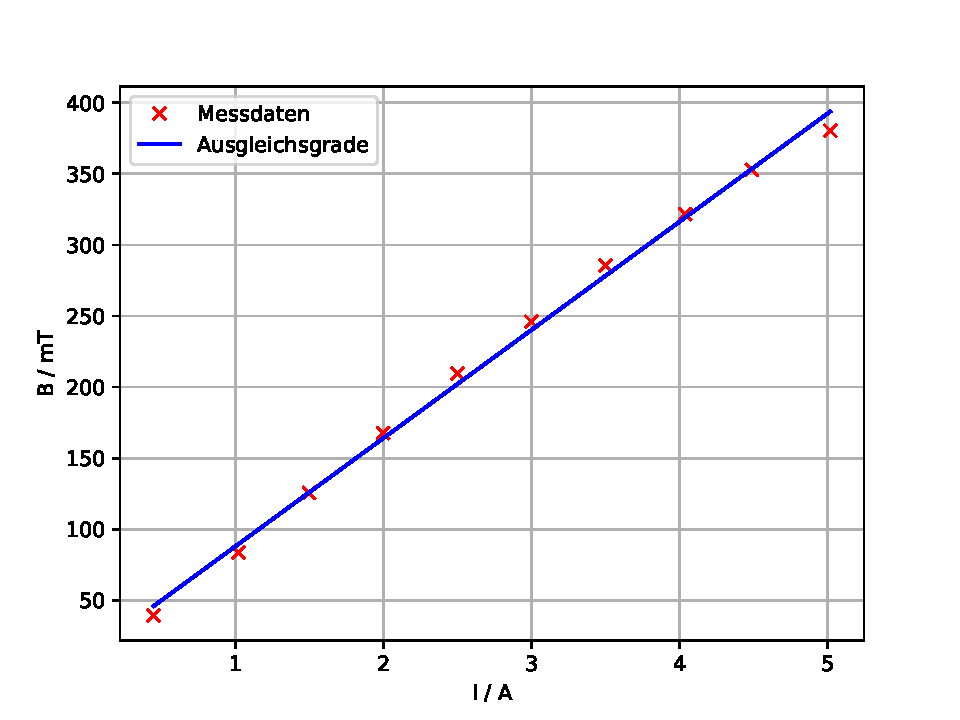
\includegraphics[width=\textwidth,keepaspectratio]{figure/B_plot.pdf}
    \caption{Messdaten und Ausgleichsgerade für die Bestimmung der Magnetfeldstärke in Abhängigkeit der Stromstärke.}
    \label{fig:Magnetfeldstärke}
\end{figure}
\FloatBarrier
\subsection{Aufspaltung der roten Spektrallinie}
Die Aufspaltung der roten Spektrallinie ist in Abbildung \ref{fig:rot_ohne_B}zu sehen.
Die Abstände $\Delta S$ und $\delta S$ werden mit dem Programm Inkscape \cite{Inkscape} vermessen.
\FloatBarrier
\begin{figure}
    \centering
    \subfloat[][]{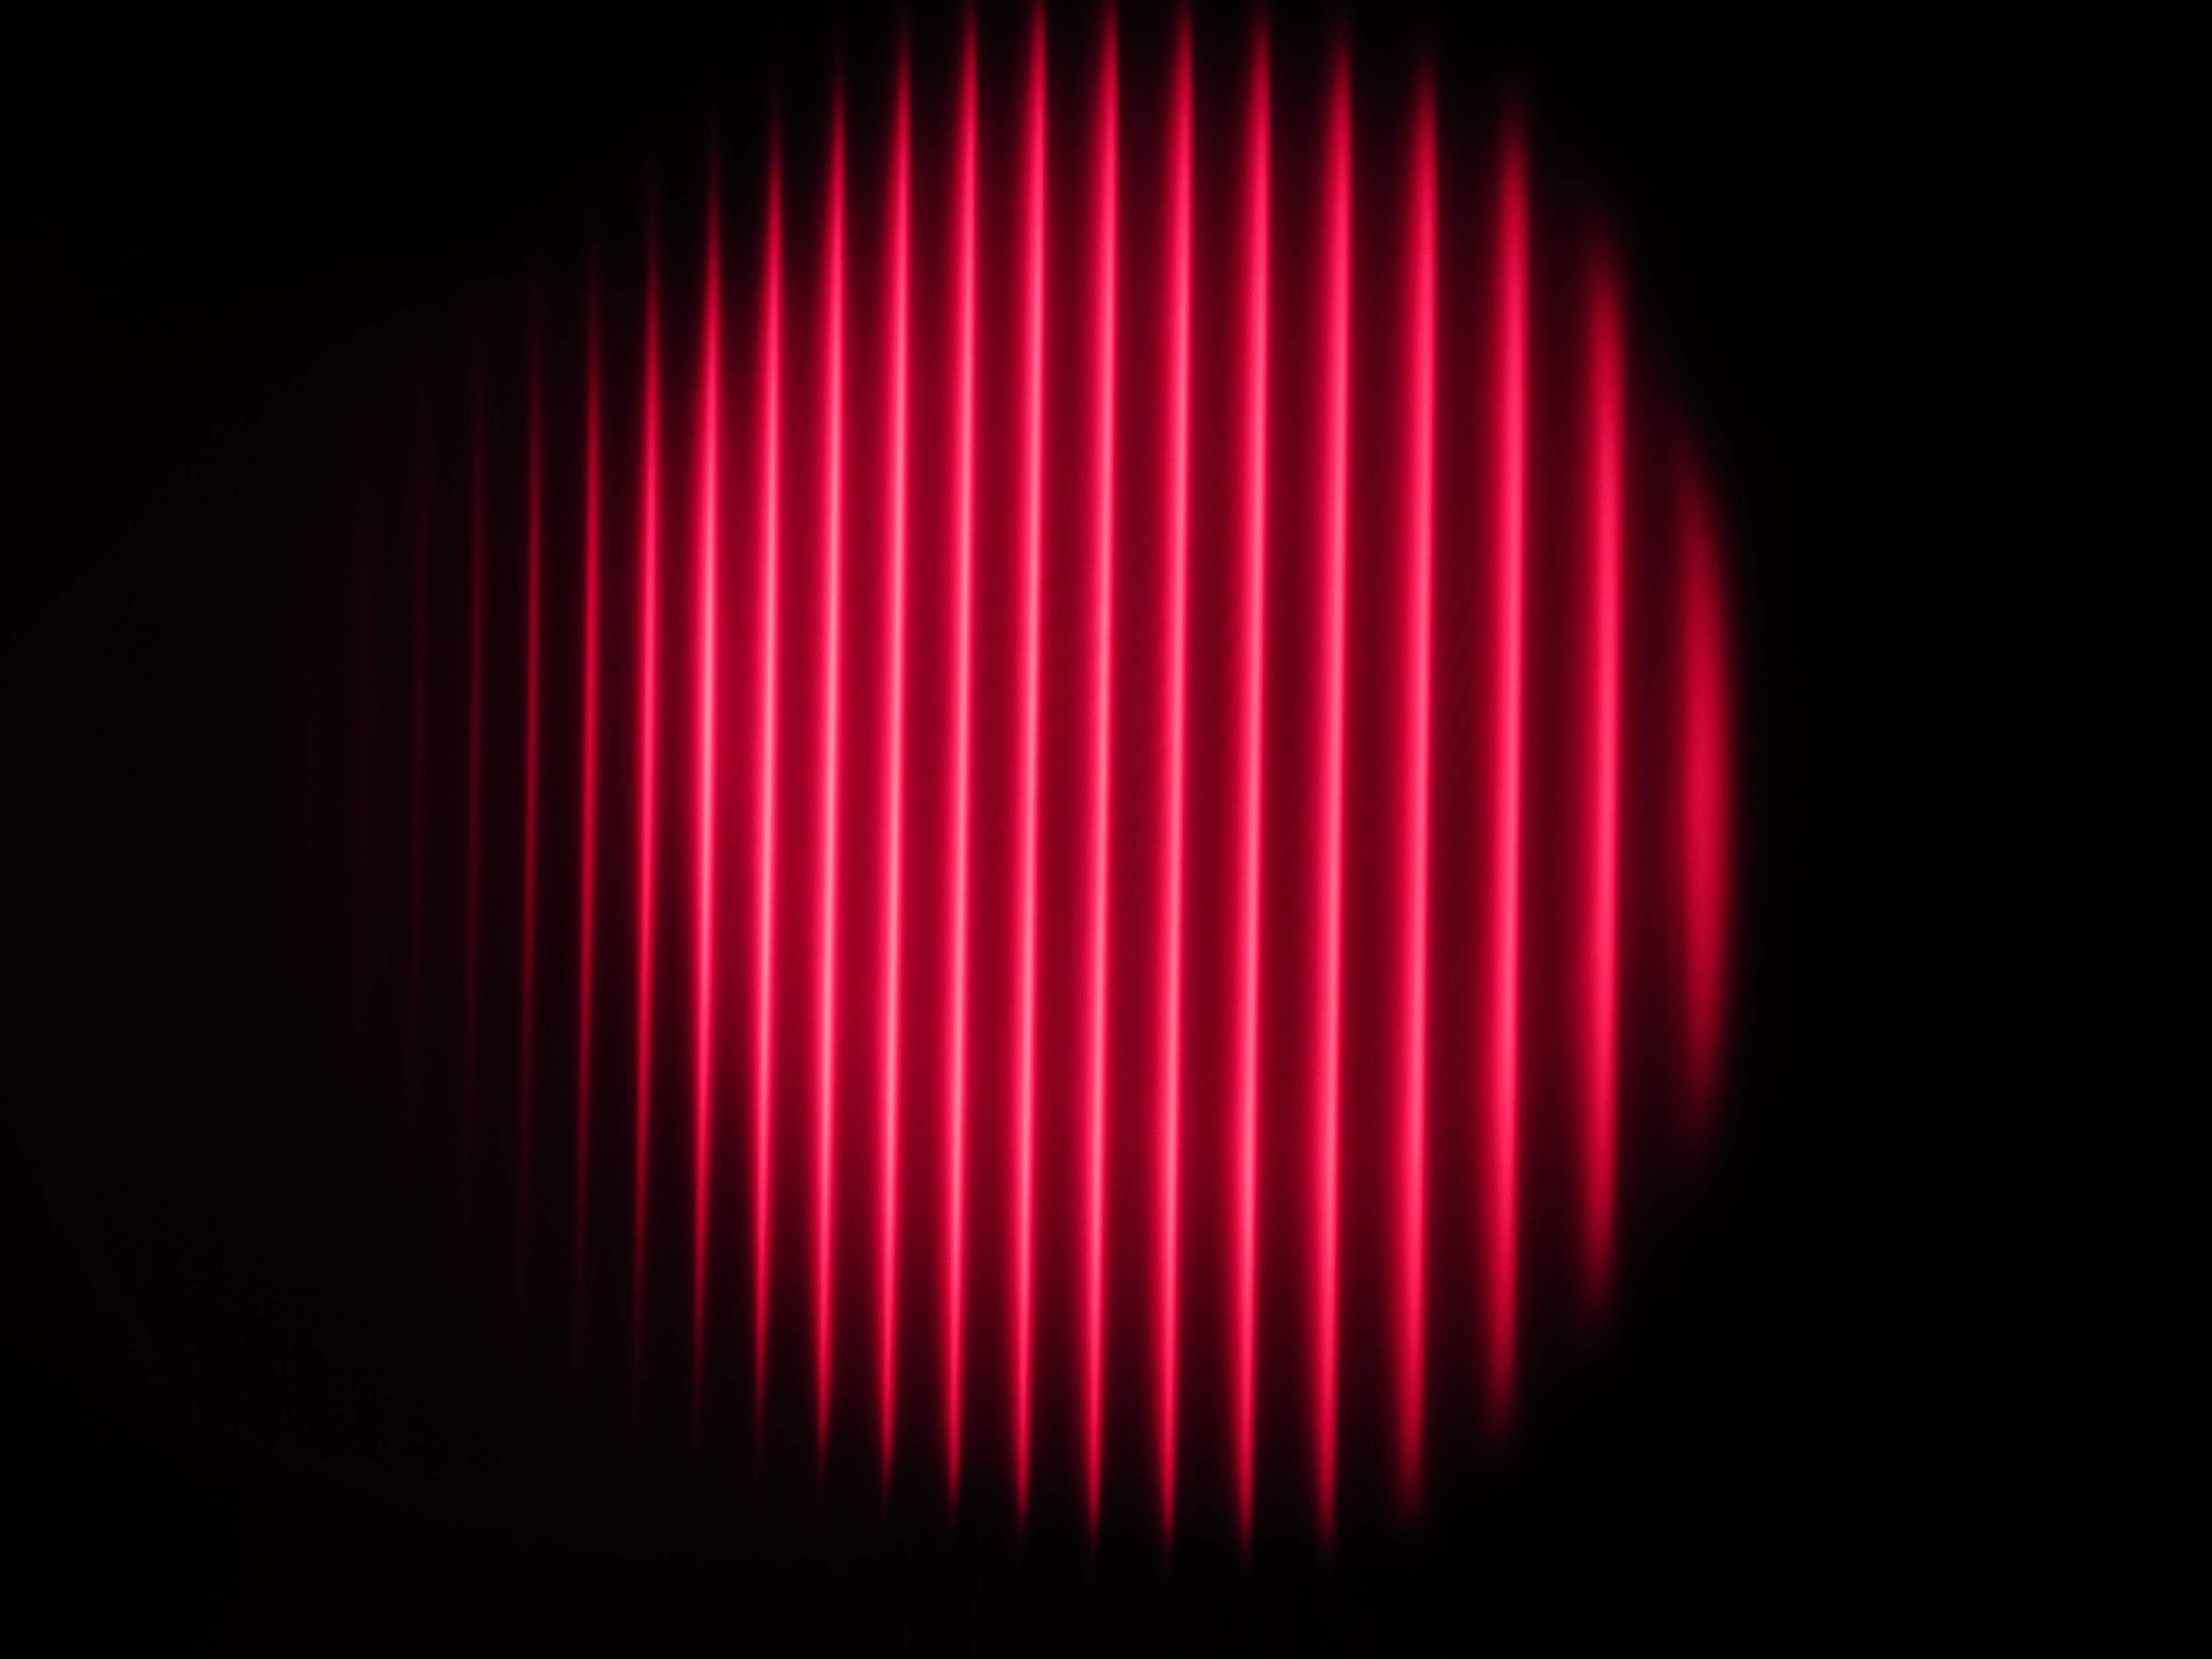
\includegraphics[width=0.45\textwidth,keepaspectratio]{../Bilder/95.pdf}}
    \vspace{0.1\textwidth}
    \subfloat[][]{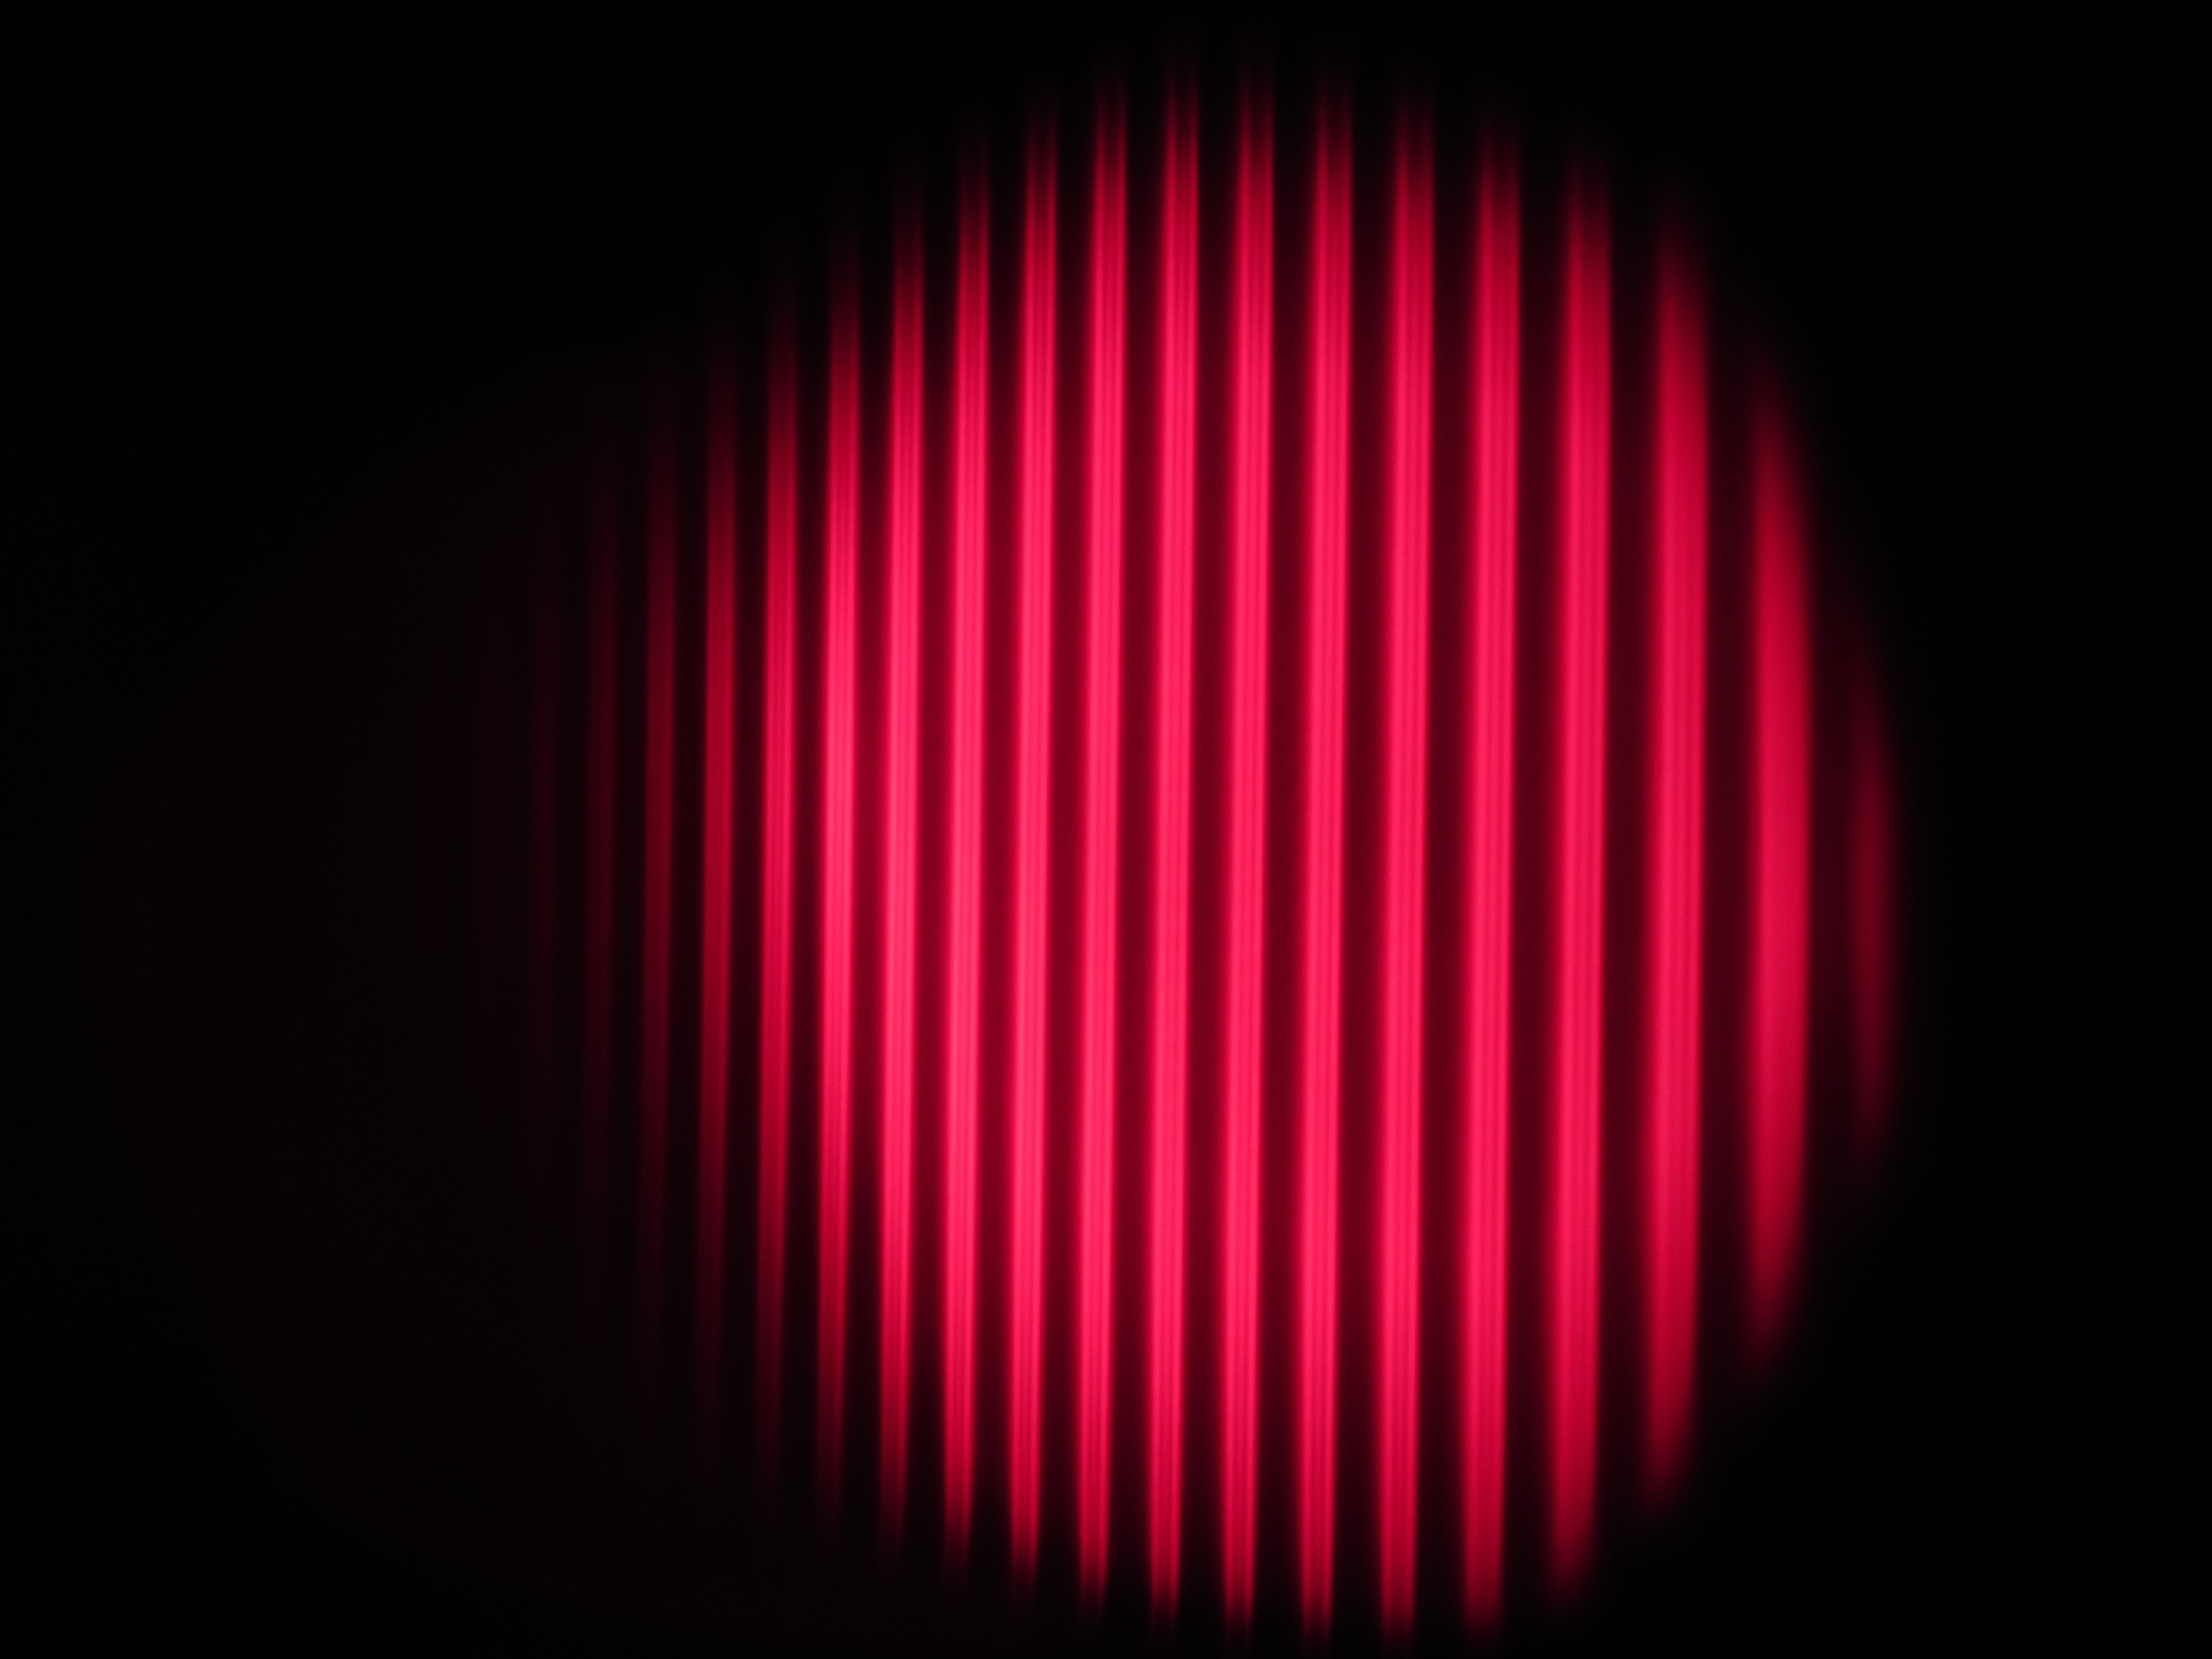
\includegraphics[width=0.45\textwidth,keepaspectratio]{../Bilder/97.pdf}}
    \caption{Messung der roten Spektrallinie für die Bestimmung der Verschiebung $\delta \lambda$ des $\sigma$-Übergangs, (a) ohne Magnetfeld, (b) mit Magnetfeld der Stärke $\SI{394(9)}{\milli\tesla}$.}
    \label{fig:rot_ohne_B}
\end{figure}
\FloatBarrier
Die Verschiebungen können mit der Formel 
\begin{equation}
    \label{eq:Verschiebung}
    \delta \lambda = \frac{1}{2}\frac{\delta S}{\Delta S}\Delta \lambda_{\text{D}} 
\end{equation}
bestimmt werden.
Die Verschiebungen und die benötigten Messwerte sind in Tabelle \ref{tab:rot_Verschiebung} aufgelistet.
\FloatBarrier
\begin{table}
    \centering
    \caption{Messwerte für die Bestimmung der Verschiebung $\delta \lambda$ der roten Spektrallinie und die $\delta\lambda$ Werte. Hierbei werden die $\Delta S$ und $\delta S$ Werte in Pixeln angegeben.}
    \label{tab:rot_Verschiebung}
    \begin{tabular}{c c c}
        \toprule
        $\Delta S$&$\delta S$&Verschiebung $\delta \lambda$ / $\SI{}{\pico\meter}$\\
        \midrule 
        $\num{61.23}$&$\num{29.96}$&$\num{11.96}$\\
        $\num{59.92}$&$\num{23.97}$&$\num{9.78}$\\
        $\num{57.53}$&$\num{28.76}$&$\num{12.22}$\\
        $\num{55.14}$&$\num{29.99}$&$\num{13.3}$\\
        $\num{63.52}$&$\num{33.64}$&$\num{12.95}$\\
        $\num{57.53}$&$\num{29.96}$&$\num{12.73}$\\
        $\num{62.32}$&$\num{35.95}$&$\num{14.1}$\\
        $\num{63.53}$&$\num{31.16}$&$\num{11.99}$\\
        $\num{67.12}$&$\num{31.18}$&$\num{11.36}$\\
        $\num{70.71}$&$\num{35.97}$&$\num{12.44}$\\
        $\num{71.91}$&$\num{35.57}$&$\num{12.09}$\\
        $\num{74.31}$&$\num{38.37}$&$\num{12.62}$\\
        $\num{77.90}$&$\num{40.77}$&$\num{12.8}$\\
        $\num{83.89}$&$\num{45.56}$&$\num{13.28}$\\
        $\num{86.29}$&$\num{50.35}$&$\num{14.27}$\\
        $\num{97.08}$&$\num{45.56}$&$\num{11.47}$\\
        \bottomrule
    \end{tabular}
\end{table}
\FloatBarrier
Aus den $\delta\lambda$ Werten aus der Tabelle \ref{tab:rot_Verschiebung} kann der Mittelwert
\begin{equation*}
    \overline{\delta\lambda} = \SI{13(1)}{\pico\meter}
\end{equation*}
für den $\sigma$-Übergang berechnet werden.
\subsection{Aufspaltung der blauen Spektrallinie}
Auch die Aufspaltung der blauen Spektrallinie wird wie im vorherigen Kapitel vermessen.
Hierbei kann allerdings ein $\sigma$ und ein $\pi$ Übergang gemessen werden.
Die Abbildungen für die Bestimmung des $\sigma$-Übergangs sind in Abbildung \ref{fig:blau_sigma} zu sehen.
\FloatBarrier
\begin{figure}
    \centering
    \subfloat[][]{
\includegraphics[width=0.45\textwidth,keepaspectratio]{../Bilder/105.pdf}}
    \vspace{0.1\textwidth}
    \subfloat[][]{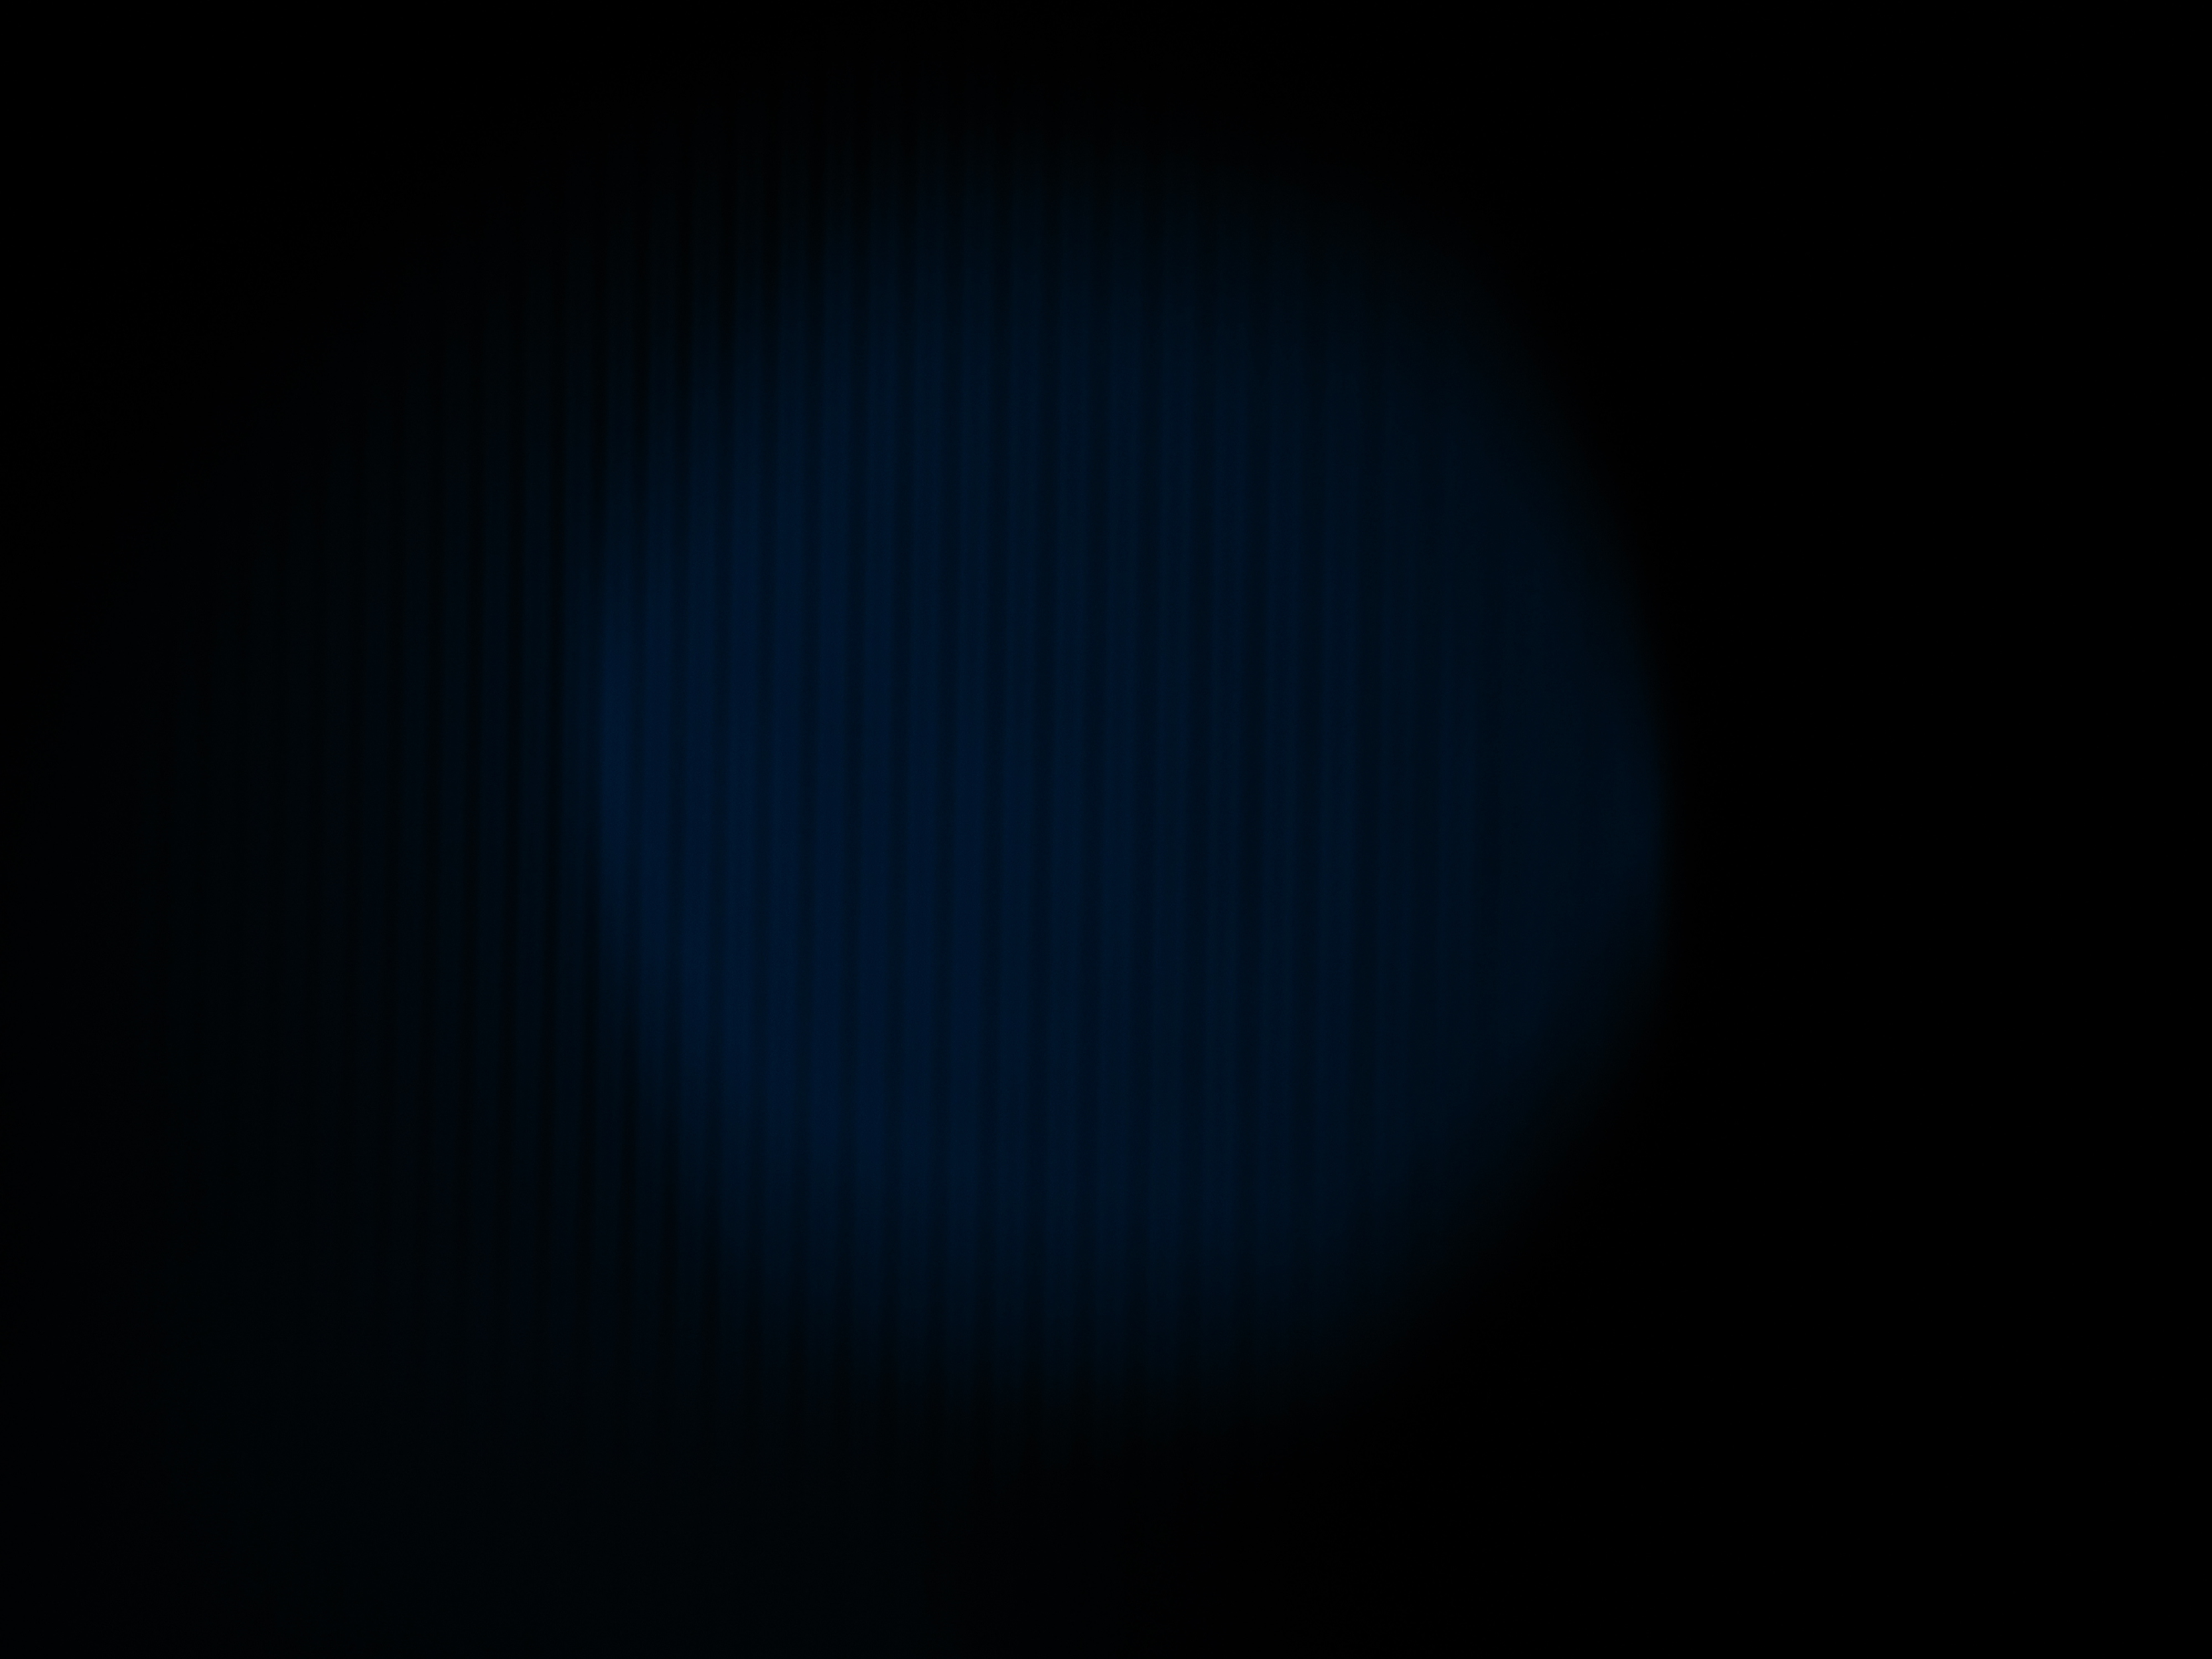
\includegraphics[width=0.45\textwidth,keepaspectratio]{../Bilder/107.pdf}}
    \caption{Messung der blauen Spektrallinie für die Bestimmung der Verschiebung $\delta \lambda$ des $\sigma$-Übergangs, (a) ohne Magnetfeld, (b) mit Magnetfeld der Stärke $\SI{313(8)}{\milli\tesla}$.}
    \label{fig:blau_sigma}
\end{figure}
\FloatBarrier
Die Messwerte sind in Tabelle \ref{tab:blau_sigma} aufgelistet. Mit der Gleichung \eqref{eq:Verschiebung} kann wieder
die Verschiebung der Wellenlänge bestimmt werden.
\FloatBarrier
\begin{table}
    \centering
    \caption{Messwerte für die Bestimmung der Verschiebung $\delta \lambda$ der blauen Spektrallinie und die $\delta\lambda$ Werte des $\sigma$-Übergangs. Hierbei werden die $\Delta S$ und $\delta S$ Werte in Pixeln angegeben.}
    \label{tab:blau_sigma}
    \begin{tabular}{c c c}
        \toprule
        $\Delta S$&$\delta S$&Verschiebung $\delta \lambda$ / $\SI{}{\pico\meter}$\\
        \midrule 
        $\num{37.29}$&$\num{26.28}$&$\num{9.51}$\\
        $\num{46.62}$&$\num{27.12}$&$\num{7.85}$\\
        $\num{39.84}$&$\num{23.73}$&$\num{8.04}$\\
        $\num{42.38}$&$\num{23.74}$&$\num{7.56}$\\
        $\num{40.69}$&$\num{28.83}$&$\num{9.57}$\\
        $\num{44.08}$&$\num{23.73}$&$\num{7.27}$\\
        $\num{49.22}$&$\num{27.13}$&$\num{7.44}$\\
        $\num{48.31}$&$\num{29.67}$&$\num{8.29}$\\
        $\num{44.10}$&$\num{24.58}$&$\num{7.52}$\\
        $\num{51.70}$&$\num{27.13}$&$\num{7.08}$\\
        $\num{50.03}$&$\num{30.51}$&$\num{8.23}$\\
        $\num{51.70}$&$\num{24.59}$&$\num{6.42}$\\
        $\num{53.39}$&$\num{30.52}$&$\num{7.72}$\\
        $\num{54.26}$&$\num{29.67}$&$\num{7.38}$\\
        $\num{56.80}$&$\num{28.81}$&$\num{6.85}$\\
        $\num{57.63}$&$\num{33.94}$&$\num{7.95}$\\
        $\num{57.63}$&$\num{29.67}$&$\num{6.95}$\\
        \bottomrule
    \end{tabular} 
\end{table}
\FloatBarrier
Die gemittelten $\delta \lambda$ Werte aus der Tabelle \ref{tab:blau_sigma} ergeben 
\begin{equation*}
    \overline{\delta\lambda} = \SI{7.7(8)}{\pico\meter}
\end{equation*}
für den $\sigma$-Übergang der blauen Spektrallinie.
Die Abbildungen für den $\pi$-Übergang sind in Abbildung \ref{fig:blau_pi} zu sehen.
\FloatBarrier
\begin{figure}
    \centering
    \subfloat[][]{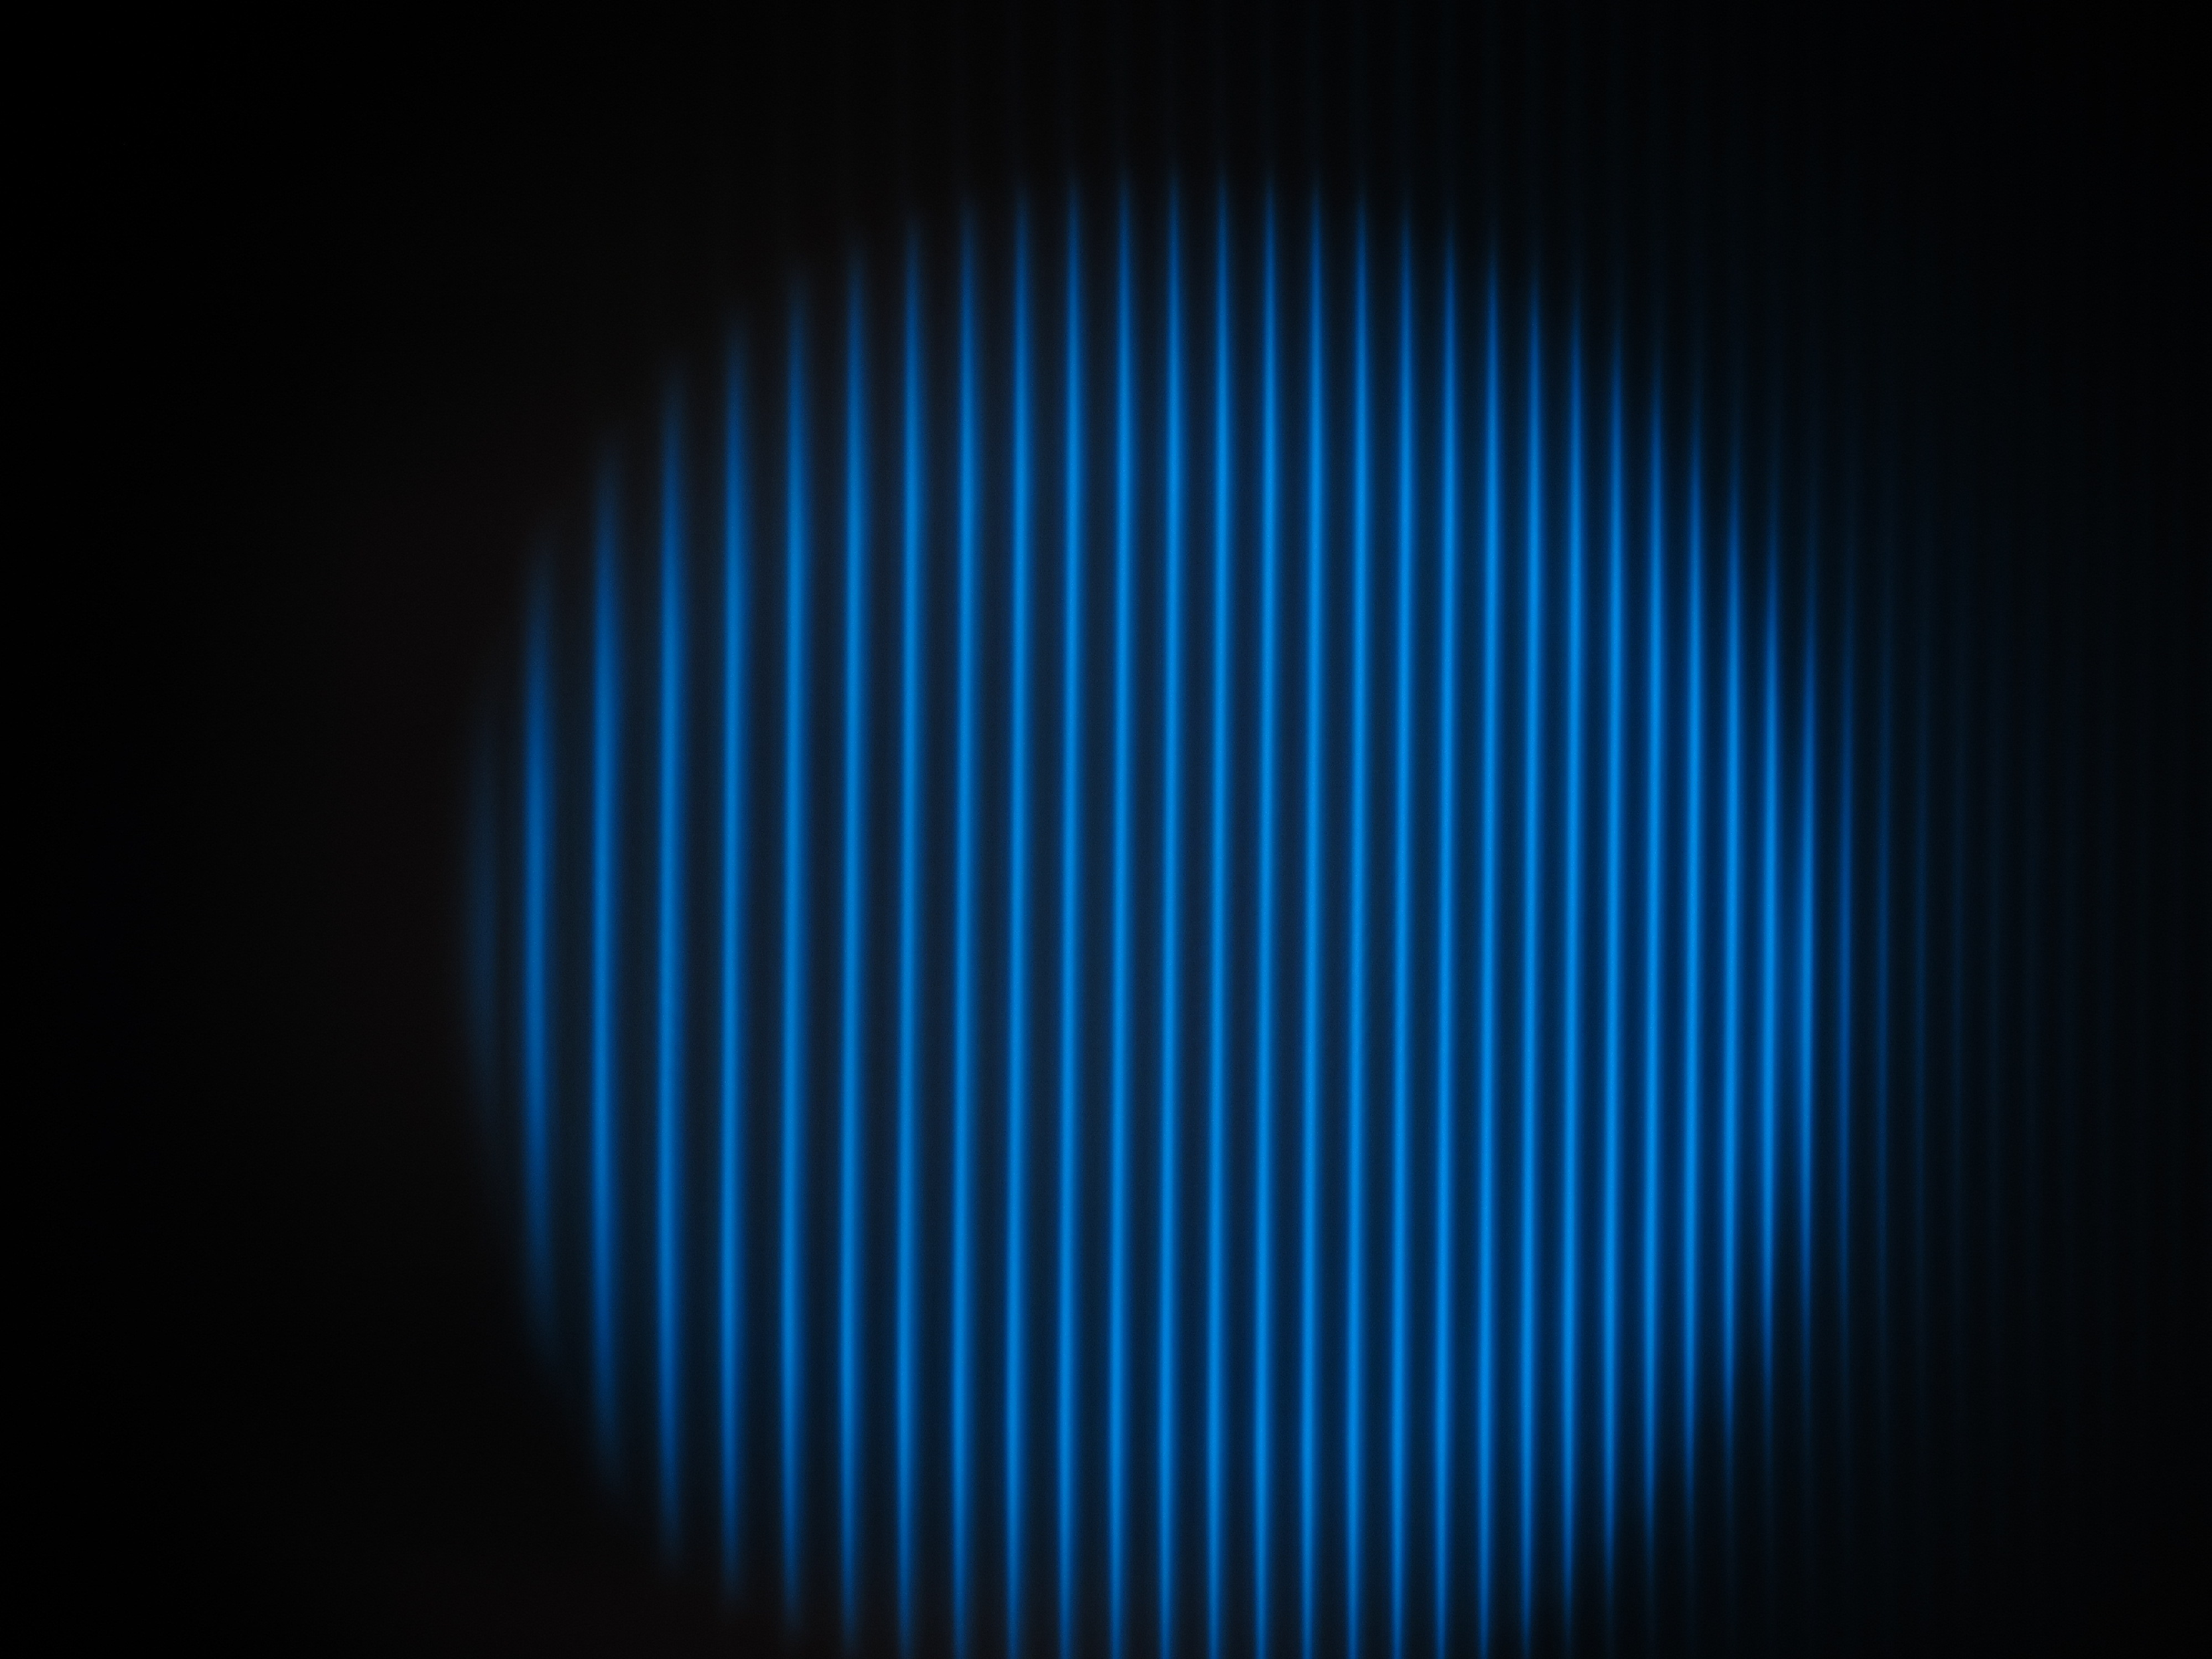
\includegraphics[width=0.45\textwidth,keepaspectratio]{../Bilder/blau_B0.pdf}}
    \vspace{0.1\textwidth}
    \subfloat[][]{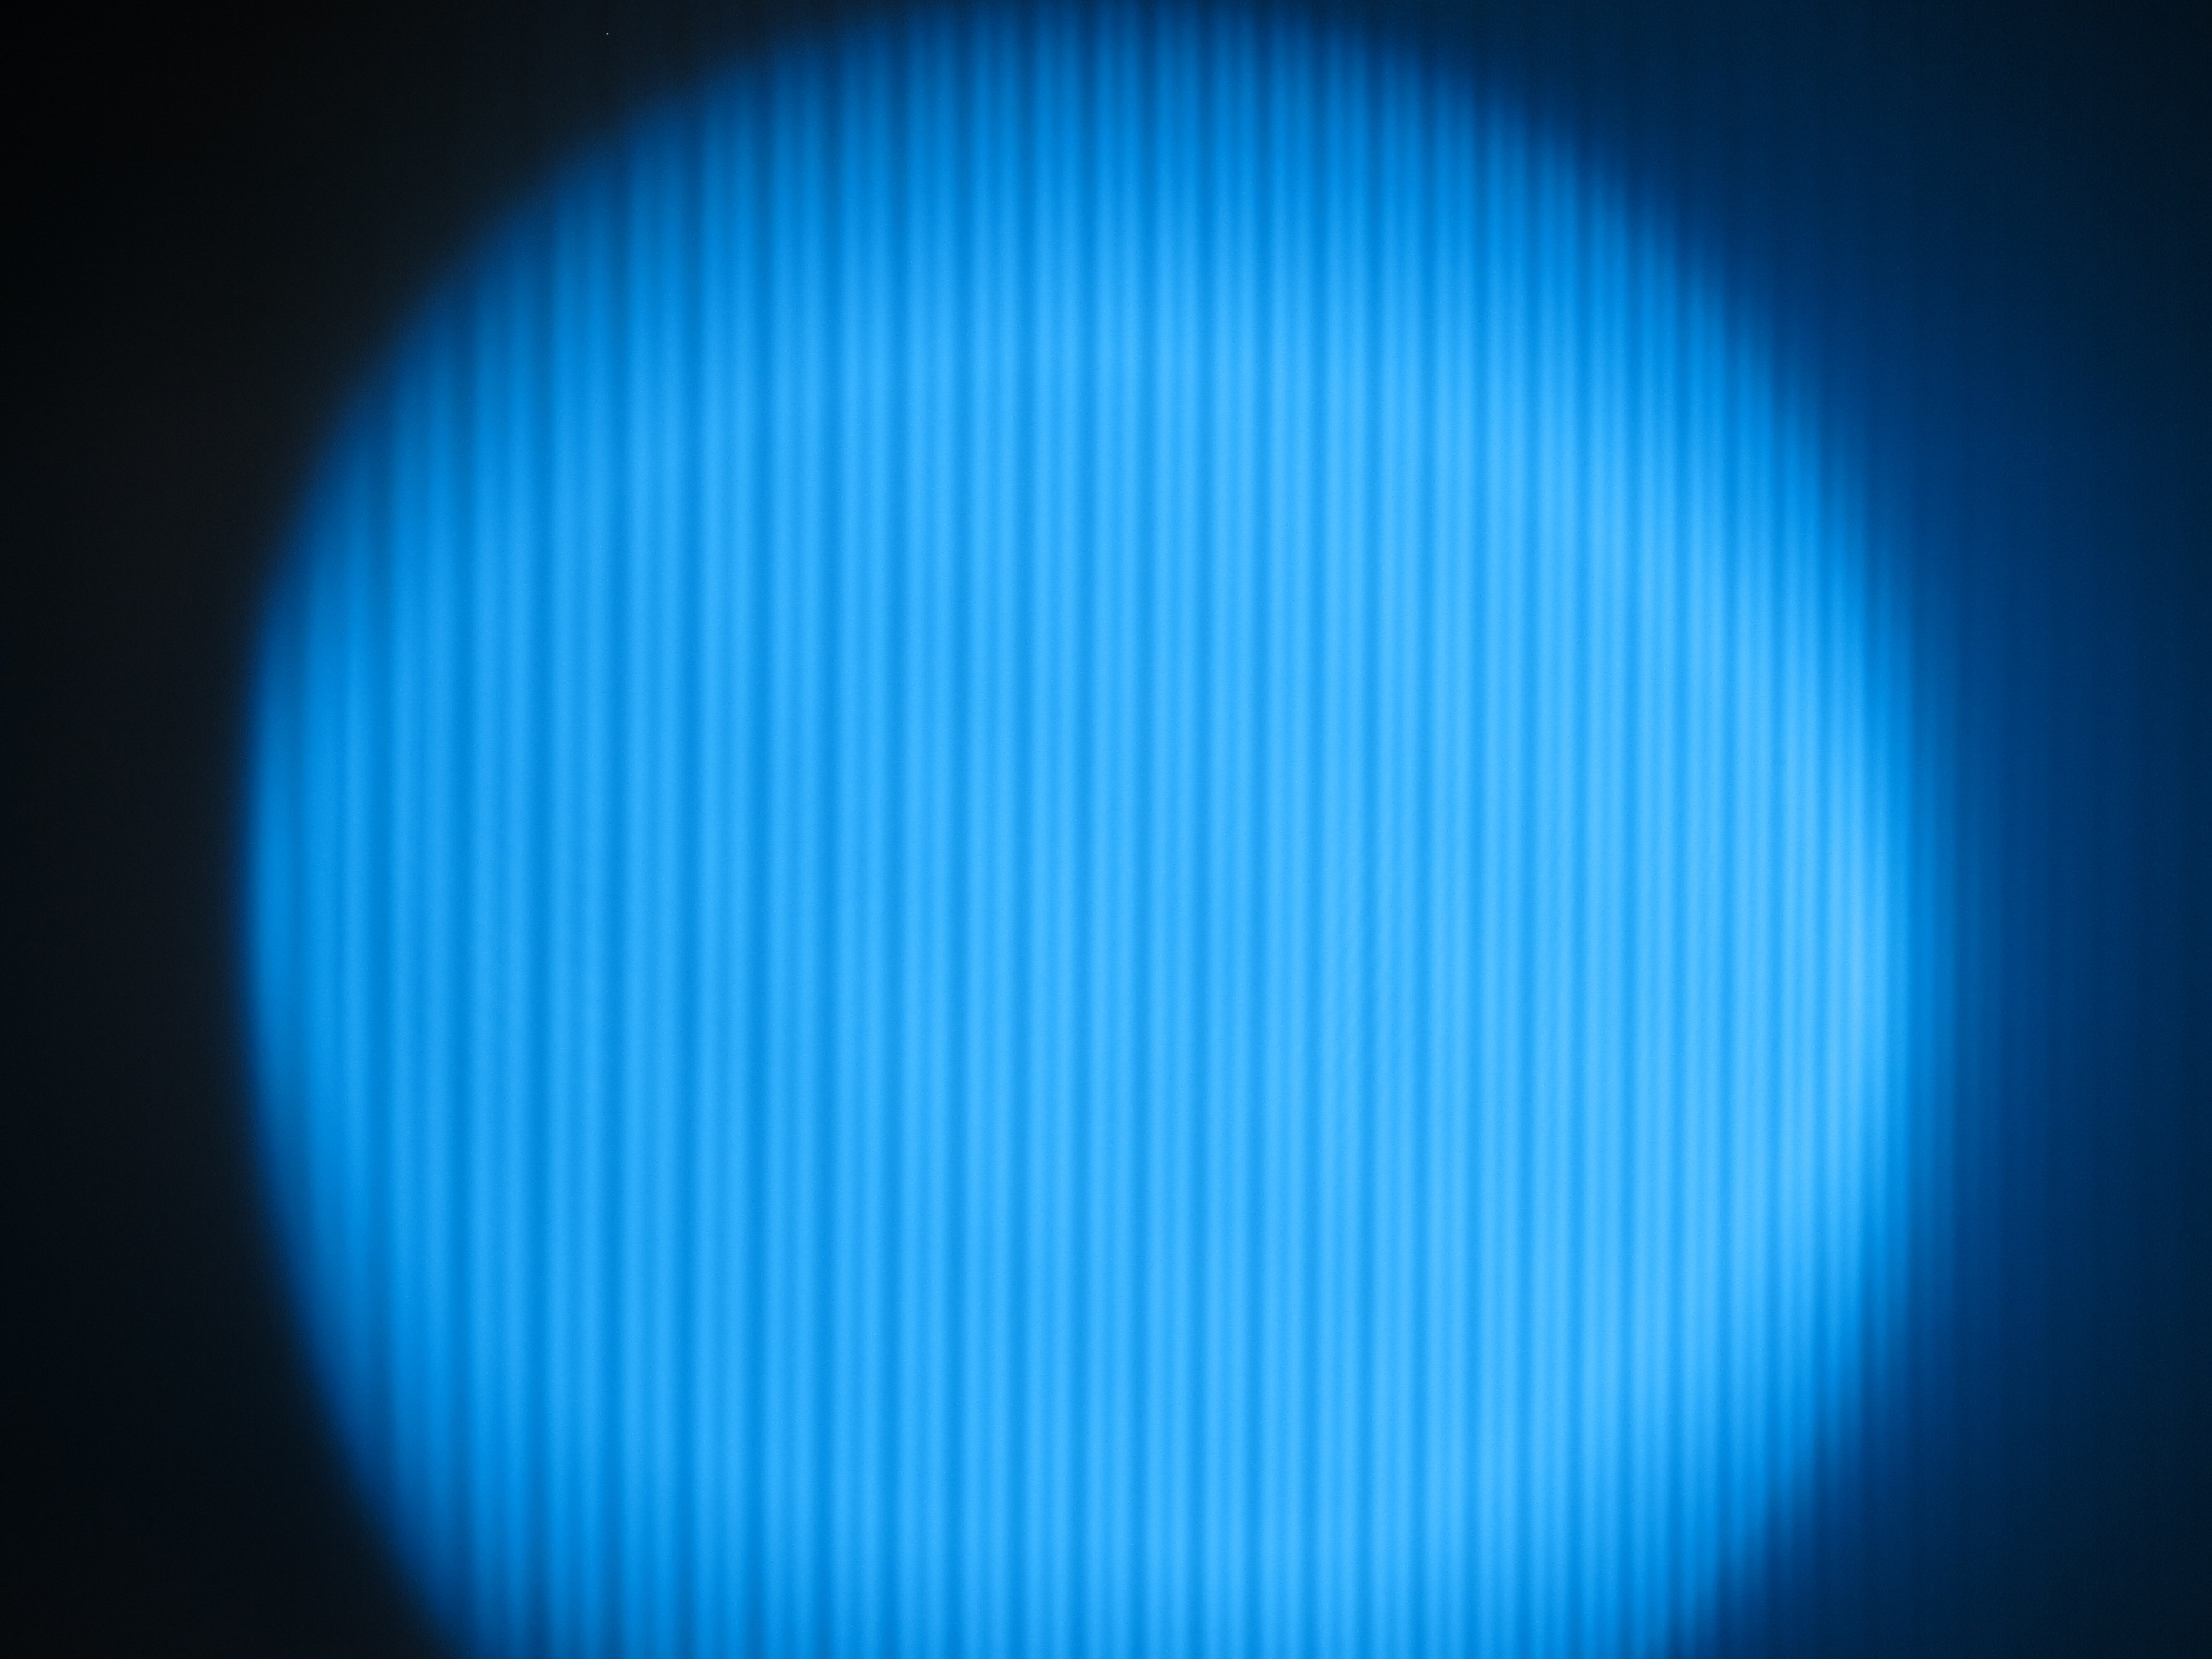
\includegraphics[width=0.45\textwidth,keepaspectratio]{../Bilder/blau_B1009_pi.pdf}}
    \caption{Messung der blauen Spektrallinie für die Bestimmung der Verschiebung $\delta \lambda$ des $\pi$-Übergangs, (a) ohne Magnetfeld, (b) mit Magnetfeld der Stärke $\SI{1009}{\milli\tesla}$.}
    \label{fig:blau_pi}
\end{figure}
\FloatBarrier
Die Messwerte für die Bestimmung der Wellenlängenverschiebung des $\pi$-Übergangs der blauen Spektrallinie sind in 
Tabelle \ref{tab:blau_pi} aufgelistet.
\FloatBarrier
\begin{table}
    \centering
    \caption{Messwerte für die Bestimmung der Verschiebung $\delta \lambda$ der blauen Spektrallinie und die $\delta\lambda$ Werte des $\pi$-Übergangs. Hierbei werden die $\Delta S$ und $\delta S$ Werte in Pixeln angegeben.}
    \label{tab:blau_pi}
    \begin{tabular}{c c c}
        \toprule
        $\Delta S$&$\delta S$&Verschiebung $\delta \lambda$ / $\SI{}{\pico\meter}$\\
        \midrule 
        $\num{57.63}$&$\num{49.14}$&$\num{11.51}$\\
        $\num{61.02}$&$\num{52.73}$&$\num{11.67}$\\
        $\num{61.92}$&$\num{41.95}$&$\num{9.15}$\\
        $\num{60.18}$&$\num{44.34}$&$\num{9.95}$\\
        $\num{59.33}$&$\num{44.34}$&$\num{10.09}$\\
        $\num{57.63}$&$\num{41.96}$&$\num{9.83}$\\
        $\num{55.94}$&$\num{38.35}$&$\num{9.26}$\\
        $\num{52.55}$&$\num{33.56}$&$\num{8.62}$\\
        $\num{51.70}$&$\num{37.15}$&$\num{9.7}$\\
        $\num{50.85}$&$\num{37.15}$&$\num{9.86}$\\
        $\num{47.49}$&$\num{32.38}$&$\num{9.2}$\\
        $\num{47.47}$&$\num{35.58}$&$\num{10.12}$\\
        $\num{49.16}$&$\num{35.95}$&$\num{9.87}$\\
        $\num{44.07}$&$\num{38.35}$&$\num{11.75}$\\
        $\num{44.92}$&$\num{35.95}$&$\num{10.8}$\\
        $\num{44.08}$&$\num{32.36}$&$\num{9.91}$\\
        $\num{43.23}$&$\num{32.38}$&$\num{10.11}$\\
        $\num{41.56}$&$\num{31.16}$&$\num{10.12}$\\
        $\num{39.97}$&$\num{28.76}$&$\num{9.71}$\\
        $\num{43.22}$&$\num{29.96}$&$\num{9.36}$\\
        $\num{39.83}$&$\num{29.99}$&$\num{10.16}$\\
        $\num{40.68}$&$\num{29.99}$&$\num{9.95}$\\
        $\num{36.48}$&$\num{22.80}$&$\num{8.44}$\\
        $\num{37.33}$&$\num{28.79}$&$\num{10.41}$\\
        $\num{38.99}$&$\num{26.48}$&$\num{9.17}$\\
        $\num{34.75}$&$\num{31.18}$&$\num{12.11}$\\
        $\num{37.33}$&$\num{21.57}$&$\num{7.8}$\\
        \bottomrule
    \end{tabular} 
\end{table}
\FloatBarrier
Die gemittelten $\delta \lambda$ Werte aus der Tabelle \ref{tab:blau_pi} ergeben 
\begin{equation*}
    \overline{\delta\lambda} = \SI{10(1)}{\pico\meter}
\end{equation*}
für den $\pi$-Übergang der blauen Spektrallinie.
\subsection{Bestimmung des Landéfaktors}
Die Änderung der Energie $\Delta E$ lässt sich durch die Gleichung 
\begin{equation}
    \label{eq:Delta_E_theo}
    \Delta E = \Delta mg\mu_{\text{B}}B
\end{equation}
beschreiben. 
Diese kann auch als Ableitung der Gleichung
\begin{equation*}
    E = \frac{hc}{\lambda}
\end{equation*}
angegeben werden. 
Die Ableitung ist 
\begin{equation*}
    \frac{\partial E}{\partial \lambda}=-\frac{hc}{\lambda^2}.
\end{equation*}
Daraus folgt die Gleichung 
\begin{equation}
    \label{eq:Delta_E}
    \Delta E =\frac{\partial E}{\partial \lambda}\cdot \delta\lambda.
\end{equation}
Die Gleichung \eqref{eq:Delta_E_theo} wird mit Gleichung \eqref{eq:Delta_E} gleichgesetzt und in die Gleichung \eqref{eq:Landeübergang} eingesetzt, um diese nach $g_{\text{ij}}$ umzustellen. Da es sich um 
Energiedifferenzen handelt, wird das negative Vorzeichen vernachlässigt.
Daraus folgt
\begin{equation}
    \label{eq:g_Bestimmung}
    g_{\text{ij}}=\frac{hc}{\lambda^2}\frac{\delta \lambda}{\mu_{\text{B}B}}.
\end{equation}
Die damit bestimmten Landé-Faktoren sind in Tabelle \ref{tab:exp_lande} aufgelistet.
\FloatBarrier
\begin{table}
    \centering
    \caption{Daten für die Bestimmung der Landé-Faktoren und die bestimmten Landé-Faktoren.}
    \label{tab:exp_lande}
    \begin{tabular}{c c c c c}
        \toprule
        $\lambda$ / $\SI{}{\nano\meter}$&Übergang&$B$ / $\SI{}{\milli\tesla}$&$\delta \lambda$ / $\SI{}{\pico\meter}$&Landé-Faktoren\\
        \midrule
        rot $\num{643.8}$ &$\sigma$ &$\num{394(9)}$ &$\num{13(1)}$  &$\num{1.6(1)}$\\
        blau $\num{480.0}$&$\sigma$ &$\num{313(8)}$ &$\num{7.7(8)}$ &$\num{2.3(3)}$\\
        blau $\num{480.0}$&$\pi$    &$\num{1009}$   &$\num{10(1)}$  &$\num{0.92(9)}$\\
        \bottomrule
    \end{tabular}
\end{table}



